Section \ref{sec:traditional-distributed-computing} described the traditional
distributed computing model, where the service provider is trusted by clients,
and defined a generalized layered architecture. This chapter first describes a
threat model, identifying threats and issues of the infrastructure and platform
layers when the service provider becomes untrusted. The threat model is followed
by changes that have to be made to the traditional trust model and architecture,
integrating confidential computing and remote attestation to address the
threats and issues.

Section \ref{sec:requirements} summarizes the changes into distinct requirements
of the trusted distributed computing model, and Section \ref{sec:evaluation}
evaluates the model using the threat model previously defined.

Finally, this chapter looks at two projects that are working on implementing the
trusted distributed computing model into the Kubernetes architecture, previously
established in Section \ref{sec:example-kubernetes}.

\section{Threat Model}
\label{sec:untrusted-threat-model}

The now untrusted service providers administer the infrastructure and platform
layer defined in Section \ref{sec:traditional-architecture-overview}. In this
threat model, we will identify threats originating from the resources and
services of these two layers.

\subsection{Infrastructure Layer}

While looking at the infrastructure layer, we will also discuss why traditional
mitigations fail in protecting data from untrusted service providers.

\begin{description}
  \item[Threats from storage resources]
    Traditionally, the service provider protects storage resources by securing
    the location of the physical hardware and storage systems that provide
    application-transparent data encryption. These measures prevent external
    attackers, but not the service provider, from gaining physical and
    plain-text access to confidential data. Therefore, data encryption has to be
    implemented at application level.

  \item[Threats from networking resources]
    Networking resources offer means of communication. However, in a distributed
    computing environment, these communication channels are often untrusted as
    these resources are shared between multiple tenants. An attacker might gain
    unauthorized access to confidential data shared by an application by
    capturing data from the shared network resources. Applications sharing
    sensitive information using untrusted communication channels need to
    implement authentication, authorization, and encryption to use these
    untrusted communication channels and not leak confidential data to a
    malicious attacker that has access to the underlying network resources.
    Authentication and encryption are usually implemented using the Transport
    Level Security (TLS) protocol \cite{rfc5246}, which utilizes a trusted third
    party (the certificate authority) for authentication, and the Diffie-Hellman
    key exchange protocol to establish a shared secret for encryption.

    Typically, these implementations do not rely on infrastructure layer
    resources and are implemented in the application layer.

  \item[Threats from compute resources]
    Techniques for protecting data resting in storage and traversing networking
    resources are primarily based on cryptographic primitives, such as
    encryption and digital signatures. These primitives require a cryptographic
    key (e.g., secret key for symmetrical encryption, private keys for
    asymmetrical encryption and singing) that needs to be kept secret.
    Typically, these keys and the decrypted data are stored in a machine's
    memory while in use, making memory a prime target for attackers.

    There are two types of physical attacks related to a machine's memory,
    summarized by \citeauthor{weis2014protecting} \cite{weis2014protecting}:
    \textsb{Direct Memory Access (DMA) Attacks} exploit the design of the x86
    instruction set architecture that allows hardware subsystems to bypass the
    CPU and directly access the memory of the machine to improve performance.
    This might lead to maliciously designed DMA devices to access or modify
    memory regions that contain confidential data. As the name implies,
    \textsb{Physical Memory Extraction (PME) Attacks} directly extract data from
    the physical system memory of a machine. Examples for this type of attack
    are monitoring the memory bus of a machine, cold boot attacks, and
    exploiting persistent nonvolatile memory modules. While software and
    hardware-based mitigations to DMA attacks exist, the firmware and software
    providing these mitigations are in control of the service provider. A
    malicious service provider could modify the firmware and software components
    to only pretend to mitigate those threats.

    One primary benefit that virtualization brings is isolation with the goal of
    shielding a VM from other VMs. Traditionally, the hypervisor is a trusted
    high-privileged software component responsible for the virtualization of
    virtual CPUs, mapping of a VM's virtualized physical memory address space to
    the host machine's physical memory address space, intercepting and carrying
    out privileged operations invoked by a VM, and providing VM management tasks
    such as starting, stopping, suspending, restoring, and migrating VMs. But a
    malicious administrator or an attacker who gained access to hypervisor level
    privileges by exploiting vulnerabilities can completely monitor and modify
    resources available to another VM that may contain confidential data. Over
    the years, many vulnerabilities have been found in commonly used hypervisors
    that break the isolation promises of hypervisors
    \cite{perezbotero2013hypervisorvulnerabilities,
      reuben2007surveyvirtualmachinesecurity}. We will refer to this kind of
    attacks as \textsb{Virtualization-based Attacks}.

    Measures for protecting VMs from the hypervisor mostly separate the
    high-privileged operations into separate components that control the access
    to these operations and move the rest of the hypervisor into a less
    privileged execution mode \cite{jin2011securevirtualization,
      szefer2012hypvervisorsecurevirtualization, li2019protectingvmfromhypervisor,
      mi2020disaggregatednestedvirtualization}. However, all of these mitigations
    are based on the trust that the party managing the hypervisor properly
    selects, configures, and patches the hypervisor. There are often no means
    for application owners to enforce or verify the selection, configuration,
    and update policies, and they are also unable to confirm that the hypervisor
    has not been tampered with.

    Aside from physical threats, \citeauthor{weis2014protecting} also describes
    the threat of \textsb{Boot Integrity (BI) Attacks}. While the application
    owner can often provide a machine's operating system, the service provider
    typically controls the firmware. BI attacks exploit the high level of
    privilege of firmware and the fact that firmware may be invisible to the
    operating system to compromise security measures in higher levels of
    software. As such, establishing trust in remote machines requires every
    piece of software executed during the machine's lifetime (including the
    firmware) to be verified or isolated.

    There have been two main approaches to preventing BI attacks:

    The \textsb{Secure Boot} approach requires each software component needed
    for the boot process, including firmware, bootloader, and kernel of the
    operating system, to be signed. During boot, the signature of these software
    components is then verified. When a software component has been modified,
    the verification fails, leading to the abortion of the boot process. This
    also requires the maintenance of a certificate which is used to verify the
    signatures. But Secure Boot does not provide means to know what specific
    components loaded during the boot process, only that those components are
    verified using the provided certificate.

    \textsb{Measured Boot} aims to provide a trusted record of the boot process.
    Traditionally, this has been done using a Trusted Platform Module (TPM),
    which contains Platform Configuration Registries (PCRs) that store
    measurements of loaded software components. Various software components,
    such as the firmware, bootloader, or kernel, take these measurements. After
    a successful boot, the PCRs are sealed, preventing the modification of the
    measurements, and signed by the TPM. Measured Boot then relies on a remote
    attestation process (see Section \ref{sec:remote-attestation}) to recover
    the signed set of measurements, verify the signature, and evaluate whether
    the measurements follow a known policy.

    Secure boot and Measured Boot rely on a trusted software component (often
    the firmware) to verify or measure other software components required for
    the boot process. However, there is no such software component in the
    traditional distributed computing model, as the service provider can modify
    all software components.
\end{description}

\begin{table}[H]
  \centering
  \scriptsize
  \begin{tabularx}{\linewidth}{
    | p{8em}
    | >{\raggedright\arraybackslash}X
    | >{\raggedright\arraybackslash}X
    | >{\raggedright\arraybackslash}X
    |
  }
  \hline
  Resource          & Threat                                      & Mitigation                                                                                              & Issue                                                                                                                               \\
  \hline
  \hline
  Storage Resources & Access of data resting in storage resources & Application level encryption of data resting in storage resources                                       &                                                                                                                                     \\
  \hline
  Network Resources & Access of data traversing network resources & Application level authentication and authorization, and encryption of data traversing network resources &                                                                                                                                     \\
  \hline
  Compute Resources & DMA attacks                                 & Software and Hardware based mitigations available                                                       & Lack of a trusted component that can verify that mitigation is working as intended                                                  \\
  \cline{2-4}
                    & PME attacks                                 &                                                                                                         & No mitigation                                                                                                                       \\
  \cline{2-4}
                    & Virtualization-based attacks                & Properly selected, configured, patched, and unmodified hypervisor                                       & Lack of trusted component that can enforce or verify the selection, configuration, update policies, and integrity of the hypervisor \\
  \cline{2-4}
                    & BI attacks                                  & Secure Boot \& \newline Measured Boot                                                                   & Lack of a trusted component that can perform measurements and/or verification                                                       \\
  \hline
\end{tabularx}

  \caption[Overview of infrastructure layer threats.]{ Overview of infrastructure
    layer threats, typical mitigations in the traditional distributed computing
    model, and arising issues when moving to the trusted distributed computing
    model. }
  \label{table:threats-overview}
\end{table}

\subsection{Platform Layer}

\begin{description}[style=standard]
  \item[Infrastructure management services] typically have full access to
    infrastructure layer resources. Therefore, the threats of the infrastructure
    layer also apply here.

  \item[Security services] offer application-level authentication,
    authorization, and encryption to support the implementation of security into
    an application. However, a malicious service provider might modify or access
    those services to use another user's credentials (Spoofing), gain privileged
    access to resources and services (Elevation of Privilege), or gain
    plain-text access to confidential data.

  \item[Monitoring and logging services] aggregate metrics and logs of
    applications. While monitoring metrics usually do not contain sensitive
    information, application logs sometimes contain sensitive information that
    can lead to the leakage of confidential data.

  \item[Application orchestration services] automate the process of preparing
    target execution environments, installing, configuring, and maintaining
    applications inside the target environments.

    A malicious service provider might misuse application orchestration services
    to leak confidential data by:

    \begin{itemize}
      \item executing malicious code in the provided target environments.
      \item modifying applications or their configurations, influencing the
            behavior of those applications.
    \end{itemize}
\end{description}

\begin{table}[H]
  \centering
  \scriptsize
  \begin{tabularx}{0.7\linewidth}{
    | p{15em}
    | >{\raggedright\arraybackslash}X
    |
  }
  \hline
  Service Type                       & Issue                                                       \\
  \hline
  \hline
  Infrastructure Management Services & Same as Infrastructure layer                                \\
  \hline
  Security Services                  & Spoofing, Elevation of Privilege, plain text access         \\
  \hline
  Monitoring \& Logging Services     & Access to possibly sensitive logs                           \\
  \hline
  Application Orchestration Services & Execution of malicious code in target execution environment \\
  \cline{2-2}
                                     & Modification of applications or their configurations        \\
  \hline
\end{tabularx}

  \caption{Overview of platform layer threats.}
\end{table}

\section{Trust Model}
\label{sec:trusted-trust-model}

The following section describe the changes made to the trust model of the
traditional distributed computing model.

The roles of the trusted distributed computing model are still present, with the
difference that the service provider is no longer considered trusted. However,
there are now three roles from the RATS framework (see Section
\ref{sec:remote-attestation}) present:

\begin{description}
  \item[Hardware Manufacturer]
    The hardware manufacturer provides hardware to the service provider that
    forms the base of the infrastructure layer. The hardware has to be able to
    create TEEs, and the hardware manufacturer endorses the security of those
    TEEs. The hardware manufacturer takes on the endorser role defined by RATS.
    Even though this model still applies when multiple TEE platforms and
    hardware manufacturers are present, for simplicity, we will assume that only
    a single TEE platform and hardware manufacturer is present.

  \item[Service Provider]
    In this model, service providers not only provide infrastructure layer
    resources and manages platform layer services but now utilize a TEE platform
    provided by the hardware manufacturer to offer the capability of creating
    TEEs and getting evidence for the integrity of the TEEs.

  \item[Reference Value Provider]
    Reference value providers generate reference values for TEEs in advance,
    which are used by the verifier to validate the integrity of TEEs created by
    the service provider.

  \item[Verifier Owner]
    An entity that operates the verifier, a new component introduced in this
    model that is responsible for assessing the trustworthiness of TEEs.

  \item[Application Owner]
    The responsibilities of application owners stayed the same. However, because
    the service provider is untrusted in this model, services of the platform
    layer are also untrusted. As such, the application owner has to ensure that
    the security of the application layer does not depend on the services of the
    platform layer.
\end{description}

The service provider is the only role that is not trusted by the data owner.
Because every other role is trusted, a single entity or organization can take on
multiple roles. However, the entity taking on the role of the service provider
can not take on any other roles.

\section{Architectural Overview}
\label{sec:trusted-architecture-overview}

\subsection{Verifier}

The verifier is a required component of the trusted distributed computing model,
responsible for verifying TEE integrity, and is operated by the verifier owner.
When a relying party, usually the application or data owner, requests the
verification of a TEE, the verifier validates that the evidence provided by the
service provider is produced by the TEE platform using endorsements from the
hardware manufacturer and verifies the integrity of the TEE using the evidence
and reference values provided by the reference value provider.

Software components involved in the creation process of TEEs, such as firmware
components of the TEE platform or VM firmware, are still under the control of
the service provider. So in order for the verifier to fully validate the
integrity of the TEE, the TEE platform's integrity also needs to be verified.

The verifier is only responsible for verifying the integrity of TEEs as a whole
and does not verify individual software and applications inside TEEs.

\subsection{Infrastructure Layer}

\begin{figure}[H]
  \centering
  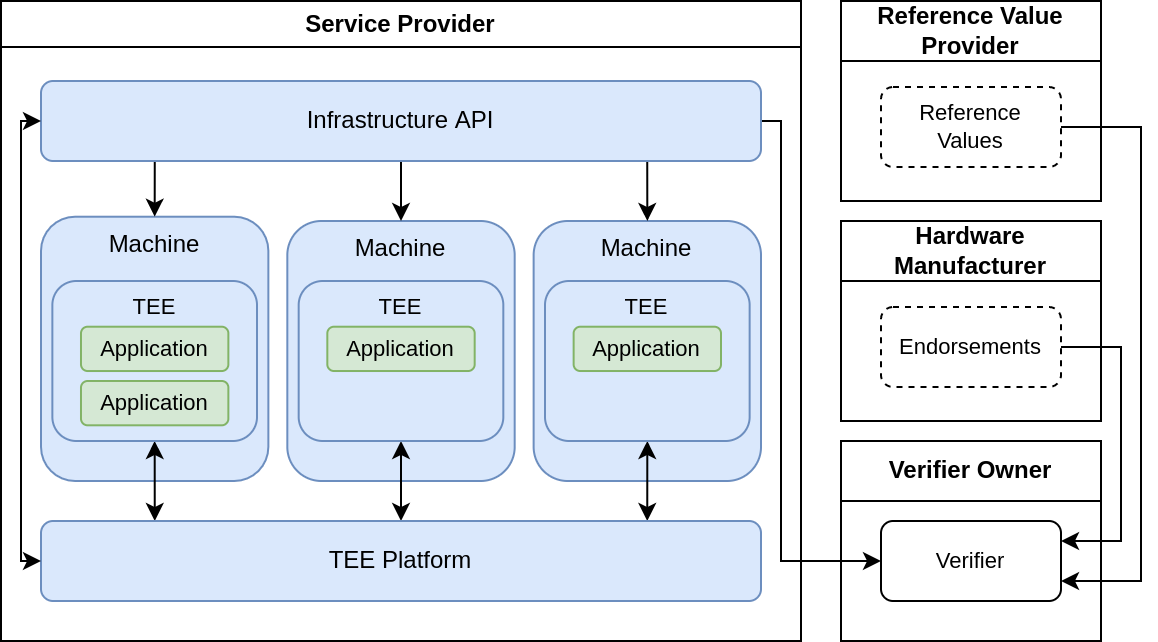
\includegraphics[width=0.9\linewidth]{resources/untrusted-infrastructure-architecture.drawio.png}
  \caption{Overview of the infrastructure layer in the trusted distributed computing model.}
  \label{fig:untrusted-architecture-overview}
\end{figure}

As outlined in the threat model, the protection of data resting in storage
resources and traversing network resources has to be implemented at the
application level using authentication, authorization, and encryption.

Instead of directly running applications on provided (physical or virtual)
machines, data and application owner rely on TEEs to protect data currently used
by applications. In Section \ref{sec:confidential-computing}, we have seen two
TEE models. On the one hand, a service provider can provide machines capable of
creating process-based TEEs inside those machines. On the other hand, a service
provider can also provide VM-based TEEs, in which case the machine itself is the
TEE.

The TEE platform has to be capable of producing evidence of software components
that have direct access or control the access to the memory of a TEE, such as
the VM firmware and firmware components of the TEE platform. The hardware
manufacturer endorses the capabilities of securely creating TEEs and producing
evidence.

A secure channel is essential for data owners to supply applications inside TEEs
with confidential data. Section \ref{sec:ra-secure-communication-channel}
outlined the basic process of establishing a secure communication channel
between the attester and the relying party during the remote attestation
process.

\subsection{Platform Layer}

Like in the traditional distributed computing model, the platform layer builds
on top of the infrastructure layer. Therefore, this section assumes the presence
of a TEE platform.

Because in this model, the service provider is untrusted, there are two possible
solutions to the threats of the services traditionally located in the platform
layer:

\begin{itemize}
  \item Moving these services to the application layer or implementing these
        services directly into applications.
  \item Splitting the service into privileged and unprivileged parts. The
        unprivileged parts can still be operated by the service provider, while
        the privileged parts have to be managed by the application owner.
\end{itemize}

The first option can be applied to all services of the platform layer.
Therefore, this section will focus on evaluating each previously defined service
category using on the latter option.

\begin{description}[style=standard]
  \item[Infrastructure Management Services] do not need to be modified and can
    still be managed by the service provider, assuming applications are
    adequately shielded from infrastructure layer resources, as described in the
    previous section.

  \item[Security Services] can not be managed by an untrusted service provider,
    as application-level security depends on those services. Management of
    identities, administration of authentication policies, and data encryption
    and decryption are privileged tasks. Therefore, splitting security services
    into unprivileged and privileged parts is not feasible and these services
    have to managed by a trusted party.

  \item[Monitoring and Logging Services] can be managed by a service provider,
    assuming that application logs do not include sensitive information or are
    protected (e.g., encrypting or obfuscating logs).

  \item[Application Orchestration Services] are a more complex topic. Because
    the TEE platform is still controlled by the untrusted service provider, the
    software responsible for managing the lifecycle of TEEs is also untrusted
    (e.g. hypervisor, OS managing process-based TEEs). An attacker can also
    modify applications and application configurations during the deployment of
    applications into TEEs. Therefore, TEEs, applications, and application
    configurations have to be verified before supplying applications with
    confidential data.

    There are two ways how to deploy applications into TEEs:

    The first option is to create an application package that the TEE platform
    can directly deploy. For example, the application owner might package an
    application, including its (non-confidential) configuration, straight into a
    VM image that the service provider can deploy as a VM-based TEE. The
    application owner has to provide reference values in the form of
    measurements of the VM to the verifier to verify the integrity of the VM,
    including the applications inside. This option moves the installation and
    configuration of applications into the application packaging process and
    therefore requires a more complex packaging solution. However, it also
    allows the combined verification of TEEs, applications, and configurations.

    The second option is to create a generic application-agnostic TEE and
    subsequently deploy the application, including its (non-confidential)
    configuration, into the TEE after verifying its integrity. For example, a
    service provider might provide a curated list of generic VM images tenants
    can deploy as VM-based TEEs. A reference value provider has to deploy such a
    VM image, check its content for malicious software, and create measurements
    of the VM beforehand, producing reference values. After a VM-based TEE is
    created, the verifier has to verify the integrity of the VM-based TEE using
    the reference values, after which the application owner installs,
    configures, and executes applications in the verified VM. This option
    decouples the creation of TEEs from the installation, configuration, and
    execution of applications, allowing another reference value provider to
    maintain reference values for TEEs. However, this also decouples the
    verification of TEEs from the verification of applications and their
    configurations, requiring two independent verifications.

    While in both cases the service provider creates TEEs, the service provider
    is not involved in the installation, configuration, and execution of
    applications in the provided TEEs. Both options also require a secure way to
    supply the applications with confidential data, which can again be achieved
    by establishing a secure communication channel during the remote attestation
    process.
\end{description}

\subsection{Application Layer}

The threat model above discussed how application-level authentication,
authorization, and encryption of confidential data are crucial to protect data
resting in storage resources and traversing network resources. As the service
provider is not trusted, infrastructure and platform layer protection methods
can not be used, and the application owner has to implement these protections
into the application layer.

As mentioned before, application logs must also be protected if they include
sensitive information. This can be achieved by encrypting application logs or
obfuscating sensitive information.

\section{Requirements}
\label{sec:requirements}

This section summarizes the changes discussed in the previous two sections by
defining requirements for the trusted distributed computing model.

The trusted distributed computing model is largely based on concepts of the
confidential computing model and requires a hardware manufacturer to provide:

\begin{enumerate}[label*=R\arabic*]
  \item a TEE platform capable of creating TEEs and generating evidence based on
        hardware mechanisms.
  \item endorsements that vouch for the TEE platform's capability to securely
        generate evidence and protect the confidentiality and integrity of TEEs.
\end{enumerate}

There are two requirements for the offerings of a service provider. The service
provider has to provide:

\begin{enumerate}[resume,label*=R\arabic*]
  \item the ability to create TEEs using the TEE platform provided by the hardware
        manufacturer.
  \item the raw evidence produced and signed by the TEE platform. This has to
        include evidence for the integrity of:
        \begin{enumerate}[label*=.\arabic*]
          \item individual TEEs.
          \item the TEE platform.
        \end{enumerate}
\end{enumerate}

The latter requirement enables the verifier to verify TEEs, preventing the
service provider to tamper with TEEs in order to break the confidentiality and
integrity guarantees. The verifier has to verify:

\begin{enumerate}[resume,label*=R\arabic*]
  \item the integrity of individual TEEs using evidence provided by the service
        provider and reference values from the reference value provider. This
        includes validating the authenticity of the evidence using the
        endorsement from the hardware manufacturer.
  \item the integrity of the TEE platform using evidence provided by the service
        provider and reference values from the hardware manufacturer. This
        includes validating the authenticity of the evidence using the
        endorsement from the hardware manufacturer.
\end{enumerate}

While TEEs protect data currently in use by applications, data resting in
storage resources and traversing network resources also have to protected. The
application management process also has to be secured, preventing the service
provider to execute malicious applications inside TEEs and modifying
applications before they are deployed into TEEs. This results in the following
requirements for the application owner. The application owner has to:

\begin{enumerate}[resume,label*=R\arabic*]
  \item implement security (authentication, authorization, and encryption) in
        the application layer, not relying on security services provided by the
        platform layer.
  \item protect application logs by removing, encrypting, or obfuscating
        confidential information from the logs.
  \item securely deploy applications inside TEEs. This includes:
        \begin{enumerate}[label*=.\arabic*]
          \item providing reference values for applications and their
                configuration.
          \item installing, configuring, and executing applications inside TEEs.
          \item supplying applications with confidential data only after
                verification of applications and their surrounding TEE (e.g., by
                establishing a secure communication channel during the remote
                attestation process).
        \end{enumerate}
\end{enumerate}

%%%%%%%%%%%%%%%%%%%%%%%%%%%%%%%%%%%%%%%%%%%%%%%%%%%%%%%%%%%%%%%%%%%%%%%%%%%%%%%%
% Evaluation
%%%%%%%%%%%%%%%%%%%%%%%%%%%%%%%%%%%%%%%%%%%%%%%%%%%%%%%%%%%%%%%%%%%%%%%%%%%%%%%%

\section{Evaluation}
\label{sec:evaluation}

This section evaluates the requirements of the trusted distributed computing
model based on the threat model defined in section
\ref{sec:untrusted-threat-model}.

Infrastructure layer threats from storage and network resources are addressed in
the trusted distributed computing model by R7. Implementing authentication,
authorization, and encryption in the application layer prevents attackers that
have access to storage and network resources from gaining plain-text access to
confidential data.

Threats from compute resources of the infrastructure layer are addressed by
R1-R6. The issue of traditional mitigations of these threats was the lack of a
trusted component that performs measurements and verification. R3 and R4 require
the service provider to offer the capability to create TEEs and get evidence
about its integrity by facilitating a TEE platform. The TEE platform is provided
and endorsed by the hardware manufacturer (R1 and R2). The TEE platform takes on
the role of the trusted component performing measurements, while verification is
performed by the verifier.

Physical access to a machine's memory is prevented as data leaving the CPU is
encrypted before storing it in memory. As such, attackers with access to the
physical memory of a machine still does not have plain-text access to the data,
preventing DMA and PME attacks.

The TEE platform also mitigates virtualization-based attacks. VM-based TEEs
split off the hypervisor's memory access control and isolation tasks into the
TEE platform. The hypervisor is still provided with interfaces to manage VMs
(e.g., starting, stopping, suspending), but the TEE platform implements the
isolation guarantee. And while the hypervisor is also tasked with managing VM
memory (e.g., attaching and releasing), the hypervisor can not read the memory
as it is encrypted.

Measurements produced by the TEE platform can also be used for the measured boot
process mitigating BI attacks against VM-based TEEs. Ongoing work in QEMU, an
open source emulator that can facilitate hardware-assisted virtualization in
order to run VMs, the open virtual machine firmware (OVMF), and the Linux kernel
enable the verification of all components involved in the boot process of an AMD
SEV-based VM \cite{decentriq2022amdsevboot}. The basic boot process works as
follows: When a VM is started, the AMD-SP measures the VM's firmware (OVMF),
which in turn measures and verifies the integrity of the Linux kernel. After the
VM has booted, the Linux kernel is supplied with an attestation report that
contains a measurement of OVMF, which is relayed to the verifier in order to
verify OVMF's integrity. The attestation report also includes evidence on the
integrity of SEV's firmware components, fulfilling requirement R4 and allowing a
verifier that supports the verification of SEV's attestation report to fulfill
R5 and R6.

The TEE creation capability of process-based TEE platforms can often be passed
through to VMs (e.g., Intel SGX), in which case the VM itself and the hypervisor
are not considered trusted. Again, isolation is provided by the TEE platform and
not the hypervisor. In this model, compromising the VM on which the
process-based TEE is deployed only threatens the availability of the application
and not the confidentiality of the application's data, mitigating
virtualization-based, and BI attacks.

R7 requires the implementation of security mechanisms in the application layer.
These mechanisms can not be based on security services provided by the platform
layer, as this would allow spoofing and elevation of privilege attacks or
plain-text access to confidential data from the untrusted service provider.
While R8 does not require moving monitoring and logging services into the
application layer, it does require the application layer to protect sensitive
information in application logs.

Application orchestration still relies on untrusted software to manage target
execution environments for applications. In this model the target environments
are VM-based TEEs managed by a hypervisor or process-based TEEs managed by the
surrounding host (or guest) OS. R9 requires that the application owner controls
the rest of the application orchestration process, that is, installation,
configuration, and execution of applications inside provided TEEs. It also
requires the verification of both TEEs and applications before supplying
applications with confidential data. On the one hand, verifying applications
allows the application owner to detect modifications of applications and their
configurations. On the other hand, removing the service provider from the
process of deploying applications into TEEs, prevents the service provider to
execute malicious code in TEEs.

While these requirements remove the service provider from the list of trusted
entities, the requirements also significantly increase the responsibilities of
application owners and the size of the application layer.

%%%%%%%%%%%%%%%%%%%%%%%%%%%%%%%%%%%%%%%%%%%%%%%%%%%%%%%%%%%%%%%%%%%%%%%%%%%%%%%%
% Case Studies
%%%%%%%%%%%%%%%%%%%%%%%%%%%%%%%%%%%%%%%%%%%%%%%%%%%%%%%%%%%%%%%%%%%%%%%%%%%%%%%%

\section{Case Studies}
\label{sec:case-studies}

\subsection{Case Study: Constellation}

Constellation is a project maintained by Edgeless
Systems\footnote{\url{https://docs.edgeless.systems/constellation/}}. By
extending Kubernetes, Constellation provides a platform base that includes
infrastructure management and application orchestration services (see Section
\ref{sec:example-kubernetes}) on top of the infrastructure layer provided by an
untrusted Cloud provider. Its contribution is the protection of the whole
Kubernetes cluster from underlying infrastructure layer resources by utilizing
VM-based TEEs and providing transparent network and storage encryption.

\begin{figure}[H]
  \centering
  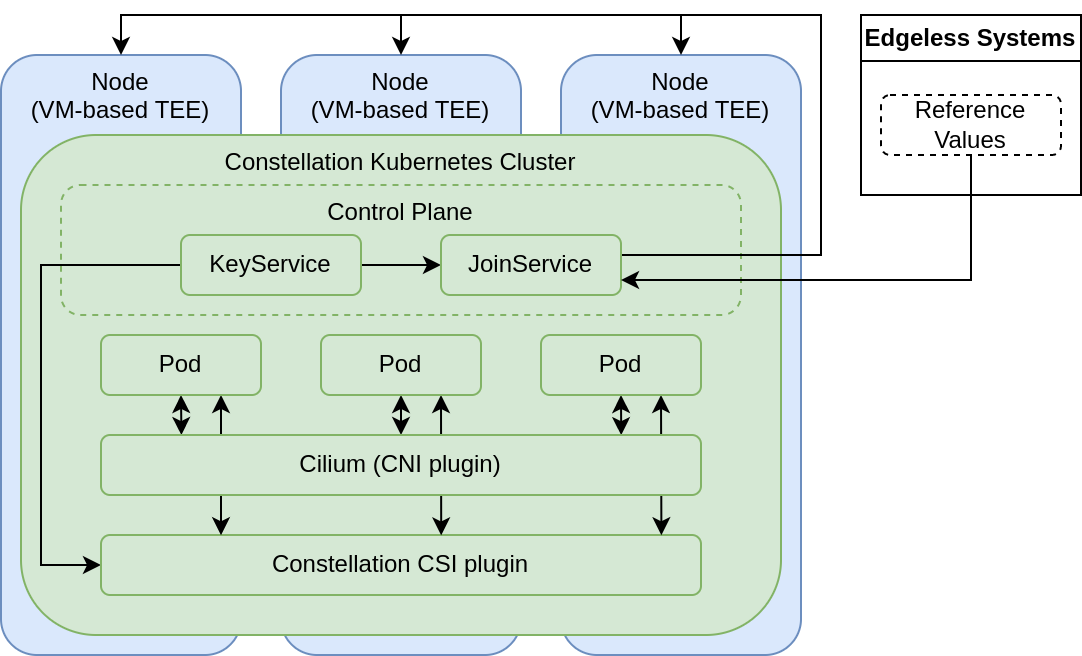
\includegraphics[width=0.8\linewidth]{resources/constellation-kubernetes.drawio.png}
  \caption{Constellation Kubernetes overview.}
\end{figure}

To protect data currently in use by control plane components and application
pods, Constellation runs the whole cluster on VM-based TEEs. The JoinService, a
new component of the control plane, is responsible for verifying new nodes
joining the cluster. After a node that is supposed to run control plane
components is verified and joins the cluster, it is supplied by the JoinService
with encryption keys which are managed by the KeyService. These keys are then
used to encrypt etcd data stored on the node, protecting control plane data at
rest.

In this architecture, the JoinService correlates to the verifier introduced
previously. It uses reference values provided by Edgeless Systems in order to
verify joining nodes. The KeyService manages cryptographic keys used for
encryption and decryption and is, therefore, a security service.

Protection of control plane and application data in transit is provided by
cilium, the CNI plugin chosen by constellation, which encrypts data exchanged
between pods without the need for applications running inside pods to be
modified. Persistent application data at rest is shielded by the CSI plugin
provided by Constellation, which encrypts and decrypts persistent volumes using
keys provided by the KeyService without needing modification of the applications
inside pods. Both the CNI and the CSI plugin are implementations of
infrastructure and security services.

Constellation currently only supports AMD SEV, making AMD take on the role of
hardware manufacturer that provides and endorses the TEE platform (R1 and R2).
However, the currently supported Cloud providers (Azure, GCP, AWS) do not fully
support the trusted distributed computing model at the time of writing. For
example, AWS currently does not provide the capability of providing SEV-based
VMs, not meeting R3. While Azure and GCP offer SEV-based VMs, Azure currently
does not facilitate reviewable VM firmware, not meeting R4.2, and GCP does not
provide evidence produced by the SEV platform, not fulfilling R4.

Because the Cloud providers do not meet R3 and R4, the JoinService (verifier)
can not meet R5 and R6. On the one hand, if the Cloud provider does not meet R3,
there are no TEEs to be verified, making complying with R5 impossible. On the
other hand, if the Cloud provider does not satisfy R4, the verifier can not
fully verify the integrity of the TEE platform or individual TEEs, preventing
the verifier from satisfying R5 and/or R6.

While Edgeless Systems provides application owners with tools to create and
manage a Constellation Kubernetes cluster, the cluster still has to be
administered by the application owner, putting the whole cluster into the
application layer. Constellation meets requirements R7 and R9, because security,
infrastructure management, and application orchestration services are all part
of the Kubernetes cluster, managed by the application owner.

\subsection{Case Study: Confidential Containers}

Confidential Containers is another project trying to implement the untrusted
distributed computing model into the Kubernetes
architecture\footnote{\url{https://github.com/confidential-containers/documentation}}.
The main difference is that while Constellation applies confidentiality at the
node level, Confidential Containers applies confidentiality at a pod level. By
running containers inside TEEs (both VM-based and process-based) and not the
whole cluster, Confidential Containers goal is to separate the trust model of
the Kubernetes cluster from the applications deployed in the cluster. The
project is still in a very early development stage, and the information provided
in this section is subject to change.

The current Kubernetes architecture puts the container runtime in charge of
managing pods and containers inside the pod (see Section
\ref{sec:example-kubernetes}). Confidential Containers introduces a new
component into the pod: the enclave agent. The enclave agent collects claims
generated by the TEE platform, performs the remote attestation process, receives
confidential configuration and data, pulls container images from the container
image registry, and manages the lifecycle of containers inside the pod. In the
case of VM-based TEEs, a pod is represented by a single VM, which includes the
enclave agent as a process that is started at boot, and the containers are
started inside the VM. For process-based TEEs, the enclave agent is a separate
process-based TEE that creates distinct process-based TEEs for each container on
the node itself. In this case study, we will illustrate the Confidential
Container architecture only using VM-based TEEs.

\begin{figure}[H]
  \centering
  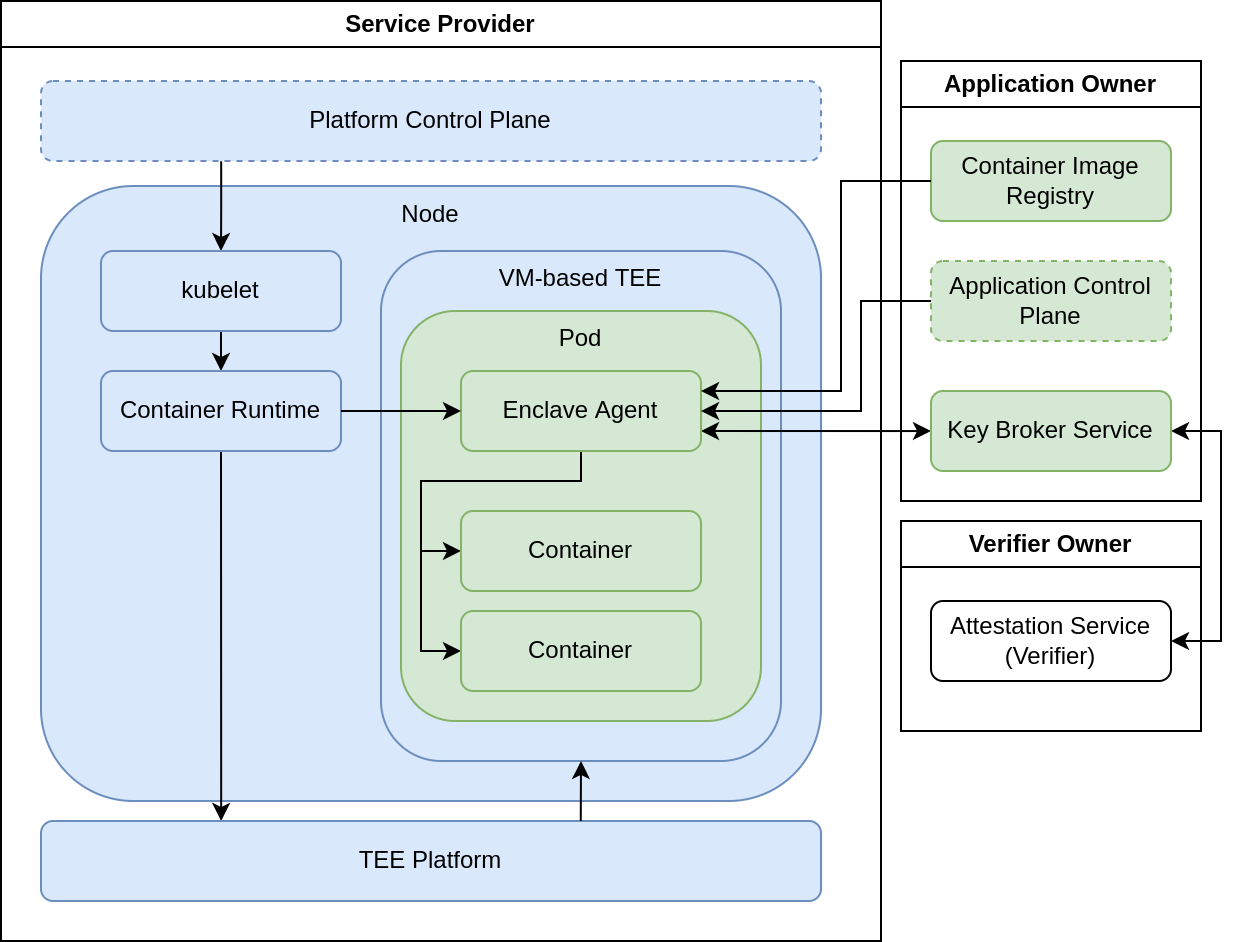
\includegraphics[width=0.8\linewidth]{resources/confidential-containers.drawio.png}
  \caption{Confidential Containers application orchestration overview.}
\end{figure}

While the agent only acts upon request from a single API source, traditionally
the Kubernetes control plane, Confidential Containers is currently working on
splitting the Kubernetes control plane into a trusted and untrusted part. The
platform control plane (untrusted) would be responsible for unprivileged tasks,
such as infrastructure and TEE management. On the other hand, the application
control plane (trusted) performs privileged tasks, including container
management inside TEEs provided by the platform control plane. The enclave agent
enforces the split of the control plane by blocking privileged actions
originating from the platform control plane, such as creating containers in a
pod and establishing a secure communication channel to the application control
plane.

The architecture builds upon the assumption that confidential data is provided
to the pod using persistent volumes managed by a CSI plugin but stored in an
encrypted form. Decryption keys are provided to pods by the key broker service,
which correlates to the relying party of the RATS framework. It receives
evidence from the enclave agent, relays the evidence to the verifier (called
attestation service in the Confidential Containers architecture) for
verification, applies appraisal policies on the returned attestation results,
and releases keys to the enclave agent. During the remote attestation process, a
secure communication channel between the key broker service and the enclave
agent is established, which is used to securely release keys to the enclave
agent. Besides data decryption keys, the key broker service also sends
communication keys to the enclave agent that are used to establish secure
communication with other components, such as the application control plane.

It is still unclear, how the ConfigMap and Secret resources of the traditional
Kubernetes architecture fit into this new architecture, which is why the
following illustration of the application orchestration process does not include
ConfigMaps and Secrets.

\begin{enumerate}
  \item Upon request of a tenant, the platform control plane requests the
        kubelet of a node to create a pod and provides the kubelet with the
        specification of the pod. This specification mainly includes container
        images, storage configuration, and network configuration.
  \item Kubelet calls the container runtime to create the pod and configure its
        storage and network.
  \item The container runtime calls the TEE platform to create a VM-based TEE
        using a predefined VM image that includes the enclave agent.
  \item During the boot of the VM, the TEE platform produces signed evidence that
        is then passed to the enclave agent after the VM has fully booted. The
        container runtime also passes the pod specifications to the enclave
        agent.
  \item The enclave agent requests the release of keys from the key broker
        service and includes the evidence in the request.
  \item The key broker service relays the evidence to the attestation service
        and receives an attestation result, upon which the key broker service
        applies its own appraisal policy.
  \item If the attestation is successful, the key broker service releases keys
        and a pod specification policy to the enclave agent. The policy can
        include, for example, storage and network configurations, a container
        image whitelist, and a certificate that can be used to validate the
        authenticity of container images.
  \item The enclave agent then compares the pod specification it received from
        the container runtime to the policy. If the specification passes the
        policy, the enclave agent pulls the specified container images and
        validates the signature using the certificate included in the policy.
  \item Only after passing the policy does the enclave agent create the
  containers inside the VM and provide them with decryption keys.
\end{enumerate}

Note that the enclave agent is only trusted, because it is included in the VM
image which is verified by the verifier. Modification of the enclave agent (or
any other software in the VM image) would fail the verification and lead to the
key broker service not releasing keys to the enclave agent.

While the overall architecture is there, Confidential Containers is still far
from production ready. Specific implementations are still missing or under
discussion, for example, the components of the remote attestation process,
mainly the key broker service and the enclave agent, are still under heavy
development, and implementation details of the dual control plane architecture
and the verification of pod specifications are still under discussion. These
issues require changes in the whole Kubernetes architecture, from the API down
to the container runtime. Before these issues have been resolved, Confidential
Containers does not fully meet requirement R9.
